% Created 2023-08-26 Sat 18:22
% Intended LaTeX compiler: pdflatex
\documentclass[11pt]{article}
\usepackage[utf8]{inputenc}
\usepackage[T1]{fontenc}
\usepackage{graphicx}
\usepackage{longtable}
\usepackage{wrapfig}
\usepackage{rotating}
\usepackage[normalem]{ulem}
\usepackage{amsmath}
\usepackage{amssymb}
\usepackage{capt-of}
\usepackage{hyperref}
\usepackage{siunitx, array, tikz}
\usetikzlibrary{angles, calc, quotes}
\author{Hankertrix}
\date{\today}
\title{Kinematics Cheat Sheet}
\hypersetup{
 pdfauthor={Hankertrix},
 pdftitle={Kinematics Cheat Sheet},
 pdfkeywords={},
 pdfsubject={},
 pdfcreator={Emacs 29.1 (Org mode 9.6.6)}, 
 pdflang={English}}
\begin{document}

\maketitle
\setcounter{tocdepth}{2}
\tableofcontents


\section{Definitions}
\label{sec:org90d3c48}

\subsection{Scalar quantities}
\label{sec:org8ec070d}
Scalar quantities are physical quantities that only have a magnitude and no direction. Examples of scalar quantities include time (\(\si{s}\)), speed (\(\si{ms^{-1}}\)) and temperature (\(\si{\celsius}\)).

\subsection{Vector quantities}
\label{sec:orgfeee2d9}
Vector quantities are physical quantities that have \textbf{both} a magnitude and a direction. Examples of vector quantities include velocity (\(\si{ms^{-1}}\)), acceleration (\(\si{ms^{-2}}\)) and force (\(\si{N}\)).

\subsection{Displacement (vector quantity)}
\label{sec:org17ce794}
Displacement is the change in position of an object over a time interval (\(\Delta \vec{x}\)). It is expressed using the equation below, where \(\Delta \vec{x}\) is the displacement of the object, and \(\vec{x_f}\) and \(\vec{x_i}\) are the final position and the initial position of the object respectively:

\[\Delta \vec{x} = \vec{x}_f - \vec{x}_i\]

The displacement is only concerned with the \textbf{end points}, and not the path taken by the object during the time interval.
\\[0pt]

Do note that a change in any physical quantity is always its \textbf{final} value minus its \textbf{initial} value.

\subsection{Distance (scalar quantity)}
\label{sec:org13c276f}
The distance is the length of the entire path taken by an object.

\subsection{Average velocity (vector quantity)}
\label{sec:org7d8e571}
The average velocity is the change in an object's position (\(\Delta \vec{x}\)) over a finite time interval (\(\Delta t\)). It is given by the equation below:

\[\text{Average velocity: } \Delta \vec{v}_{av} = \frac{\Delta \vec{x}}{\Delta t} = \frac{\vec{x}_2 - \vec{x}_1}{t_2 - t_1}\]

\subsection{Instantaneous velocity (vector quantity)}
\label{sec:org838aca4}
The instantaneous velocity is the velocity of an object at a specific instance of time. Mathematically, it is when the limit of the time interval becomes an infinitesimally small value. This is expressed mathematically in the equation below:

\[\text{Instantaneous velocity: } \vec{v} = \lim_{\Delta t \rightarrow 0} \frac{\Delta \vec{x}}{\Delta t} = \frac{d \vec{x}}{dt}\]

In GCE A-level texts, the instantaneous velocity is often defined to be the rate of change of displacement. However, this should not be the case and the instantaneous velocity should be defined as the rate of change of \textbf{position}.

\subsection{Speed (scalar quantity)}
\label{sec:org70b726c}
Speed is defined as the \textbf{magnitude} of velocity.

\subsection{Average acceleration (vector quantity)}
\label{sec:org77ea53b}
The average acceleration is the change in velocity over a finite time interval. This is expressed mathematically in the equation below:

\[\text{Average acceleration: } \vec{a}_{av} = \frac{\Delta \vec{v}}{\Delta t} = \frac{\vec{v}_2 - \vec{v}_1}{t_2 - t_1}\]

\subsection{Instantaneous acceleration (vector quantity)}
\label{sec:org5b1daea}
The instantaneous acceleration is the acceleration of an object at a specific instance of time. Mathematically, it is when the limit of the time interval becomes an infinitesimally small value. This is expressed mathematically in the equation below:

\[\text{Instantaneous acceleration: } \vec{a} = \lim_{\Delta t \rightarrow 0} \frac{\Delta \vec{v}}{\Delta t} = \frac{d \vec{v}}{dt} = \frac{d^2 \vec{x}}{dt^2}\]

The units of acceleration give a sense of how to understand this quantity. It is given by metres per second per second, i.e. it is the change in velocity (\(\si{ms^{-1}}\)) every second.

\subsection{Relative velocity}
\label{sec:org001656e}
The velocity of a moving body seen by a particular observer is called the velocity \emph{relative} to that observer.

\subsection{Frame of reference}
\label{sec:orgf9570b9}
A frame of reference is a coordinate system plus a timescale.

\newpage

\section{Formulas}
\label{sec:orgb74d358}

\subsection{General relations in kinematics}
\label{sec:org99df6f0}
\(\indent\) The gradient of a position-time (\(x-t\)) graph is velocity.
\[\vec{v} = \lim_{\Delta t \rightarrow 0} \frac{\Delta \vec{x}}{\Delta t} = \frac{d \vec{x}}{dt}\]

\[\Downarrow\]

The area under a velocity-time (\(v-t\)) graph is displacement.
\[\int_{\vec{x}_i}^{\vec{x}_f} \, d \vec{x} = \int_{t_i}^{t_f} \vec{v} t \, dt\]
\[\vec{x}_f - \vec{x}_i = \int_{t_i}^{t_f} \vec{v} t \, dt\]
\\[0pt]

The gradient of a velocity-time (\(v-t\)) graph is acceleration.
\[\vec{a} = \lim_{\Delta t \rightarrow 0} \frac{\Delta \vec{v}}{\Delta t} = \frac{d \vec{v}}{dt} = \frac{d^2 \vec{x}}{dt^2}\]

\[\Downarrow\]

The area under an acceleration-time (\(a-t\)) graph is acceleration.
\[\int_{\vec{v}_i}^{\vec{v}_f} \, d \vec{v} = \int_{t_i}^{t_f} \vec{a} t \, dt\]
\[\vec{v}_f - \vec{v}_i = \int_{t_i}^{t_f} \vec{a} t \, dt\]


\subsection{Equations of motion for constant acceleration}
\label{sec:orga812f0a}

\[v = v_0 + at \tag{1}\]
\[s = v_0t + \frac{1}{2} at^2 \tag{2}\]
\[v^2 = {v_0}^2 + 2as \tag{3}\]

\subsection{Relative velocity}
\label{sec:org1c8c245}
\[\vec{v}_{PA} = \vec{v}_{PB} + \vec{v}_{BA}\]

\newpage

\section{Resolving vectors}
\label{sec:org34e6ea8}
A vector can be resolved into 2 separate perpendicular vectors that are independent of each other.

\begin{center}
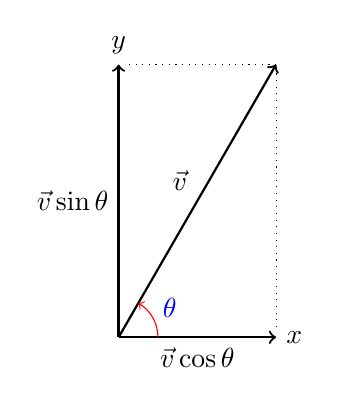
\begin{tikzpicture}

% Start of the 1st example
% Setting the origin
\coordinate (origin) at (0,0);

% Draw the original vector
\draw[thick, ->] (origin) -- ++(60:4) coordinate (vec) node[midway, above left] {$\vec{v}$};

% Draw the resolved vectors
\draw[thick, black, ->] (origin) -- ++(2,0) node (x) {} node[right] {$x$} node[midway, below] {$\vec{v} \cos \theta$};
\draw[thick, black, ->] (origin) -- ++(0,3.464101615) node (y) {} node[above] {$y$} node[midway, left] {$\vec{v} \sin \theta$};

% Draw the dotted lines
\draw[dotted, black] (y) -- ++(2,0);
\draw[dotted, black] (x) -- ++(0,3.464101615);

% Draw the angle
\pic [draw=red, text=blue, ->, "$\theta$", angle eccentricity=1.5] {angle = x--origin--vec};

\end{tikzpicture}
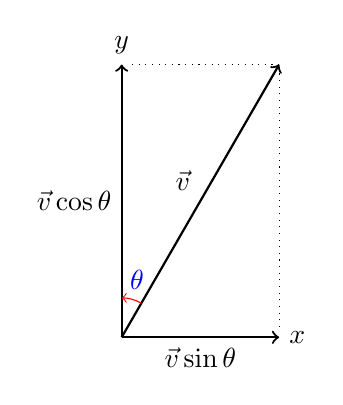
\begin{tikzpicture}

% Start of the 2nd example
% Setting the origin
\coordinate (origin) at (0,0);

% Draw the original vector
\draw[thick, ->] (origin) -- ++(60:4) coordinate (vec) node[midway, above left] {$\vec{v}$};

% Draw the resolved vectors
\draw[thick, black, ->] (origin) -- ++(2,0) node (x) {} node[right] {$x$} node[midway, below] {$\vec{v} \sin \theta$};
\draw[thick, black, ->] (origin) -- ++(0,3.464101615) node (y) {} node[above] {$y$} node[midway, left] {$\vec{v} \cos \theta$};

% Draw the dotted lines
\draw[dotted, black] (y) -- ++(2,0);
\draw[dotted, black] (x) -- ++(0,3.464101615);

% Draw the angle
\pic [draw=red, text=blue, ->, "$\theta$", angle eccentricity=1.5] {angle = vec--origin--y};

\end{tikzpicture}

\[\]

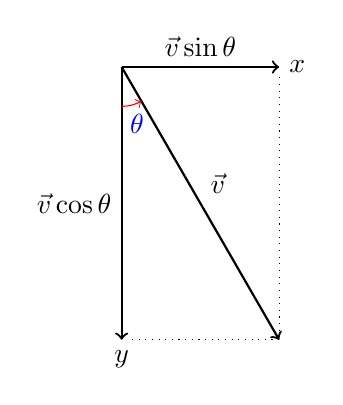
\begin{tikzpicture}

% Start of the 3rd example
% Setting the origin
\coordinate (origin) at (0,0);

% Draw the original vector
\draw[thick, ->] (origin) -- ++(300:4) coordinate (vec) node[midway, above right] {$\vec{v}$};

% Draw the resolved vectors
\draw[thick, black, ->] (origin) -- ++(2,0) node (x) {} node[right] {$x$} node[midway, above] {$\vec{v} \sin \theta$};
\draw[thick, black, ->] (origin) -- ++(0,-3.464101615) node (y) {} node[below] {$y$} node[midway, left] {$\vec{v} \cos \theta$};

% Draw the dotted lines
\draw[dotted, black] (y) -- ++(2,0);
\draw[dotted, black] (x) -- ++(0,-3.464101615);

% Draw the angle
\pic [draw=red, text=blue, ->, "$\theta$", angle eccentricity=1.5] {angle = y--origin--vec};

\end{tikzpicture}
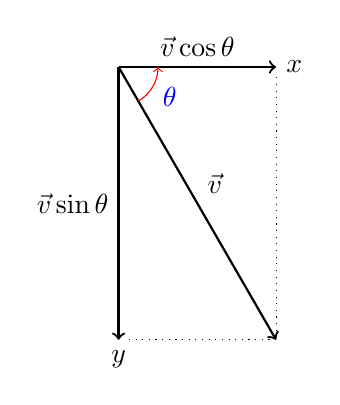
\begin{tikzpicture}

% Start of the 4th example
% Setting the origin
\coordinate (origin) at (0,0);

% Draw the original vector
\draw[thick, ->] (origin) -- ++(300:4) coordinate (vec) node[midway, above right] {$\vec{v}$};

% Draw the resolved vectors
\draw[thick, black, ->] (origin) -- ++(2,0) node (x) {} node[right] {$x$} node[midway, above] {$\vec{v} \cos \theta$};
\draw[thick, black, ->] (origin) -- ++(0,-3.464101615) node (y) {} node[below] {$y$} node[midway, left] {$\vec{v} \sin \theta$};

% Draw the dotted lines
\draw[dotted, black] (y) -- ++(2,0);
\draw[dotted, black] (x) -- ++(0,-3.464101615);

% Draw the angle
\pic [draw=red, text=blue, ->, "$\theta$", angle eccentricity=1.5] {angle = vec--origin--x};

\end{tikzpicture}

\end{center}


In general, the resolved vector \(\vec{v}_r\) that encloses the angle between the original vector \(\vec{v}\) and the resolved vector \(\vec{v}_r\) will have a magnitude of \(\vec{v} \cos \theta\). The other resolved vector will have a magnitude of \(\vec{v} \sin \theta\).

\newpage

\section{Relating acceleration to velocity}
\label{sec:org2017635}

\begin{center}
\begin{tabular}{ |m{11em}|m{11em}| }
\hline
If $x$-velocity is: & $x$-accleration is: \\
\hline
Positive \& increasing (getting more positive) & Positive: The object is moving in the $+ \, x$-direction \& speeding up \\
\hline
Positive \& decreasing (getting less positive) & Negative: The object is moving in the $+ \, x$-direction \& slowing down \\
\hline
Negative \& increasing (getting less negative) & Positive: The object is moving in the $- \, x$-direction \& slowing down \\
\hline
Negative \& decreasing (getting more negative) & Negative: The object is moving in the $- \, x$-direction \& speeding up \\
\hline
\end{tabular}
\end{center}


\section{Accelerating while maintaining a constant speed?}
\label{sec:orgf953b46}
Even when the speed of an object is constant (remember that the speed of an object is a scalar quantity), as long as the direction of the object changes, the \textbf{velocity} of the object is \textbf{changing}. This means a car has a non-zero acceleration if it rounds a bend at constant speed. Since the car's direction is changing, its \textbf{velocity} is also \textbf{changing} and hence it has \textbf{non-zero acceleration}.
\\[0pt]

Hence, you should not use the layman understanding of acceleration to mean speeding up. When there is an acceleration, it just means that the velocity is changing, which doesn't necessarily mean that the speed is changing.
\end{document}